\documentclass{acmsiggraph}
\usepackage[english]{babel}
\usepackage[T1]{fontenc}
\usepackage[latin1]{inputenc}
\usepackage{float, enumitem, footnote, multirow}
\usepackage[font=scriptsize,labelfont=bf, justification=centering, format=hang]{caption}
\usepackage{subfig}
\usepackage{amsmath, amsthm, amssymb, bbm}
\usepackage[ruled,vlined]{algorithm2e}
\usepackage{hyperref}
\usepackage{microtype}
\usepackage{lmodern}
\usepackage{listings}
\lstset{
	basicstyle=\footnotesize
}
\graphicspath{{../figures/}}
\DeclareMathOperator\sign{sign}

\newcommand\mycommfont[1]{\footnotesize\ttfamily{#1}}
\SetCommentSty{mycommfont}
\newcommand{\R}{\mathbb{R}}
\newcommand{\1}{\mathbbm{1}}
\DeclareMathOperator\sig{sigmoid}


%-----------------------
% TIKZ
% -----------------------
    \usepackage{tikz}
    \usetikzlibrary{arrows,positioning}
    \tikzstyle{circ}=[draw, circle, fill=white, align=center, inner sep=1,outer sep=0]



\title{Machine Learning for Computer Vision\\ {\large [MVA 2015/2016]}\\
\vspace{10pt}
Programming Assignment 3}

\author{Maha ELBAYAD
%\\ \texttt{maha.elbayad@student.ecp.fr}}
}
\pdfauthor{Maha ELBAYAD}
\newcommand{\E}{\mathbb{E}}
\begin{document}
\maketitle
\section{Building classifiers as neural network layers}
For each of the SVM, logistic regression and linear regression we implement a loss function to run a neural network version of the optimization algorithms. Each input $x_i$ has a score $f(x_i)$ related to the probability of the sample being  positive.

\begin{align*}
\text{(Linear regression) } & l_i = \frac{1}{2}(f(x_i)-y_i)^2\\
&  f(x_i) = w^Tx_i+b\\
\text{(Logistic regression) } & l_i = y_if(x_i)+(1-y_i)(1-f(x_i))\\
& f(x_i)= \sig(w^Tx+b)\\
\text{(SVM) } & l_i = \max(1-y_if(x_i))\\
&  f(x_i) = w^Tx_i+b
\end{align*}

\textbf{Results with different parameters $\alpha$ (leraning rate) and $\lambda$ (weight decay)}
\begin{figure}[H]
\centering
\includegraphics[width=8cm]{logit}
\caption{Logistic regression}
\end{figure}

\begin{figure}[H]
\centering
\includegraphics[width=8cm]{svm}
\caption{SVM}
\end{figure}

\begin{figure}[H]
\centering
\includegraphics[width=8cm]{lr}
\caption{Linear regression}
\end{figure}
We note that for all three models, the evolution of the loss and the final number of misclassified samples is independent from the weight decay parameter. This term is equivalent to a regularization parameter that causes the weights $w$ to exponentially decay to zero in order to avoid over-fitting the training set.\\
In the update:
\[w^i_{t+1} := w_i^t -\alpha \frac{\partial L(w)}{\partial w^i} - \alpha\lambda w_i^t\]
Since we're obliged to use small learning rate $\alpha$ for the optimization to converge, the decay term $\alpha\lambda$ is too small to be effective.\\
Best results with SVM and logistic regression were achieved with a relatively large learning rate $\alpha=$1e-2 where the learning overshoots at first before stabilizing.

\textbf{Momentum:}
\begin{equation}
w^i_{t+1} := w_i^t +\mu \Delta w_t^i-\alpha \frac{\partial L(w)}{\partial w^i} - \alpha\lambda w_i^t
\end{equation}
\label{Emom}
\begin{figure}[H]
\centering
\subfloat[Linear regression]{\includegraphics[width=8cm]{lr_mom}}\\
\subfloat[SVM]{\includegraphics[width=8cm]{svm_mom}}\\
\subfloat[Logistic regression]{\includegraphics[width=8cm]{log_mom}}
\caption{Neural networks with momentum\label{mom}}
\end{figure}

As can be seen in figure \ref{mom} and equation (\ref{Emom}), the additional momentum term allows an accelerated convergence to the minimum as it keeps track of the previous update and  take larger steps in directions of persistent reduction as well as preventing chaotic jumps (e.g. in the logistic regression we eliminated the overshooting occurring with $\mu=0$) 


\section{Sum/Max-Product algorithms}
We implement the sum-prodcut algorithm on the following undirected tree:
\begin{figure}[H]
\centering
	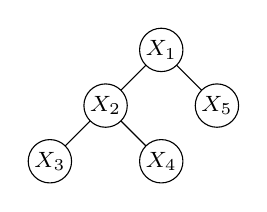
\begin{tikzpicture}[node distance=.5cm,auto,>=latex',font=\sffamily\footnotesize]
        \node [circ] (a) {$X_1$};
        \node [circ] (b) [below left of =a, node distance = 1cm] {$X_2$};
        \node [circ] (c) [below right of =a, node distance = 1cm] {$X_5$};
        \node [circ] (d) [below left of =b, node distance = 1cm] {$X_3$};
        \node [circ] (e) [below right of =b, node distance = 1cm] {$X_4$};
        \path[-] 
        (a) edge node {} (b)
        (a) edge node {} (c)
        (b) edge node {} (d)
        (b) edge node {} (e);
    \end{tikzpicture} 
\end{figure}
We first pass the messages from the leaves $\{3,4,5\}$ to their parents $\{2, 2, 1\}$ and then 2 passes its messages to the root 1, which will allow us to compute the marginal probability  $\widetilde P(X_1)$. Afterwards, we pass the messages in the opposite direction and we stop at 2 since we only need to compute $\widetilde P(X_2)$.\\
A message from node $X_i$ to $X_j$ is evaluated as:
\[\mu_{i\to j}(X_j) = \sum_{X_i}\psi_i(X_i)\psi_{i,j}(X_i,X_j)\prod_{k\in\mathcal N(i)\backslash j}\mu_{k\to i}(X_i) \]
In a similar fashion, we implement the max product algorithm (takes the maximum instead of the sum in the definition of the passed message).\\
\paragraph{Sum-product results:}
Marginal probabilities:
\[\begin{split}
\widetilde P(X_1) &= [0.5580, 1.0170, 0.3400]\\
\widetilde P(X_2) &= [0.8700, 1.0450]
\end{split}\]
Both summing to $Z = 1.9150$.
\[\begin{split}
P(X_1) &= [0.2914, 0.5311, 0.1775]\\
P(X_2) &= [0.4543, 0.5457]
\end{split}\]
We evaluate $P(X)$ on some events:
\[\begin{split}
P(X=\{1,2,4,2,1\}) &= 0.0056\\
P(X=\{3,1,2,1,2\}) &= 0.0033\\
P(X=\{2,2,1,2,1\}) &= 0.0134\\
\end{split}\]
\end{document}